\documentclass{article}
%\usepackage{ctex} %Chinese
\usepackage{float} %H-float
\usepackage{graphicx} %
\usepackage{amsmath} %
\usepackage{amssymb} %
\usepackage{amsthm} %
\usepackage{mathtools}
\usepackage{caption}
\usepackage[version=3]{mhchem}  %
\usepackage{chemfig}    %
\usepackage{physics}
\usepackage{booktabs}
\usepackage{hyperref}
%\usepackage{caption}    %
%  \captionsetup[figure]{name=Fig}
\usepackage{enumerate} %列表
\usepackage[scale=0.85]{geometry} %
\usepackage{tikz}
%\usepackage{mmap}
%\usepackage{tikz,venndiagram}
\newtheorem{theorem}{Theorem}
\newtheorem{corollary}{Corollary}[theorem]
\newtheorem{lemma}[theorem]{Lemma}

\newcommand{\sq}[1]{\ensuremath{\left[{#1}\right]}}
\newcommand{\R}[1]{\ensuremath{\mathrm{R}\!\left({#1}\right)}}
\newcommand{\kB}{\ensuremath{k_\mathrm{B}}}
\newcommand{\iu}{\ensuremath{\mathrm{i}}}
\newcommand{\dpath}[1]{\ensuremath{\mathcal{D}\!\left[{#1}\right]}}
\newcommand{\set}[1]{\ensuremath{\left\{{#1}\right\}}}
\newcommand{\kket}[1]{\ensuremath{\ket{\ket{#1}}}}
\newcommand{\ie}{\emph{i.\,e.}}

\DeclareFontFamily{OMS}{oasy}{\skewchar\font48 }
\DeclareFontShape{OMS}{oasy}{m}{n}{%
         <-5.5> oasy5     <5.5-6.5> oasy6
      <6.5-7.5> oasy7     <7.5-8.5> oasy8
      <8.5-9.5> oasy9     <9.5->  oasy10
      }{}
\DeclareFontShape{OMS}{oasy}{b}{n}{%
       <-6> oabsy5
      <6-8> oabsy7
      <8->  oabsy10
      }{}
\DeclareSymbolFont{oasy}{OMS}{oasy}{m}{n}
\SetSymbolFont{oasy}{bold}{OMS}{oasy}{b}{n}

\DeclareMathSymbol{\smallleftarrow}     {\mathrel}{oasy}{"20}
\DeclareMathSymbol{\smallrightarrow}    {\mathrel}{oasy}{"21}
\DeclareMathSymbol{\smallleftrightarrow}{\mathrel}{oasy}{"24}

\newcommand{\tensor}[1]{\overset{\scriptscriptstyle\smallleftrightarrow}{#1}}



\title{CHM452: Problem Set 3}
\author{Xinxian Chen%
\footnote{Email: \href{mailto:xchen106@ur.rochester.edu}{xchen106@ur.rochester.edu}}}
\date{\today}

\begin{document}

\maketitle

Let $\iu = \sqrt{-1}$, $o(\cdot)$ and $O(\cdot)$ are little-o and big-O notations, respectively, and $\mathbb{N}$ is the set of natural numbers ($\mathbb{N} = \set{0,\ 1,\ 2,\ 3,\ \ldots}$) and $\mathbb{N}_+ = \mathbb{N}\setminus\set{0}$

\begin{enumerate}[1.]
  \item Set $\hbar = 1$.
  \begin{enumerate}[(i)]
    \item Analytically, when $x_0 = 0$ and $p_0 = 0$,
    \begin{align*}
      \ev{x^2} &= \qty(\frac{\alpha}{\pi})^{1/2}\int_{-\infty}^{\infty} \dd{x}x^2 e^{-\alpha x^2} 
      = \qty(\frac{\alpha}{\pi} \frac{\pi}{4\alpha^3})^{1/2}
      = \frac{1}{{2\alpha}},
      \ev{x} = \qty(\frac{\alpha}{\pi})^{1/2}\int_{-\infty}^{\infty} \dd{x}x e^{-\alpha x^2} 
      = 0.
    \end{align*}
    When $\alpha = 1$, $\Delta x = \sqrt{\ev{x^2} - \ev{x}^2} = 1/\sqrt{2} \approx 0.70710678$.
  
    Use the grid basis in the range $[-20,\ 20]$ and the number of grid points be 1024, and results are:
    \begin{quotation}
      norm: $1.00000000$; $\ev{x}$: $0.00000000$; and $\Delta x$: $0.70710678$.
    \end{quotation}
    The wavefunction is plotted in Figure~\ref{fig:1-1}.
    \begin{figure}[H]
      \centering
      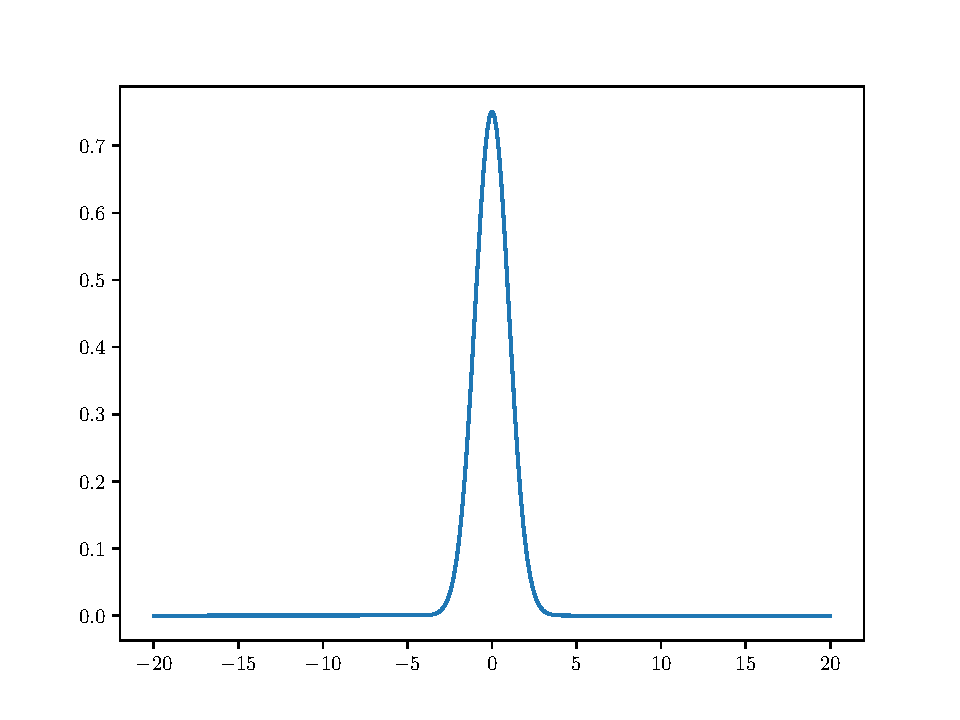
\includegraphics[width=0.6\linewidth]{q1-1.pdf}
      \caption{}
      \label{fig:1-1}
    \end{figure}

    \item Analytically, when $x_0 = 0$ and $p_0 = 0$, the fourier transformation gives
    \begin{align*}
      \Psi_0(p) &= \frac{1}{\sqrt{2 \pi }} \int \dd{x} e^{-\iu px} \Psi_0(x)
      =\frac{1}{\sqrt{2 \pi }} \qty(\frac{\alpha}{\pi})^{1/4}  \int \dd{x} e^{-\iu px -\alpha x^2/2}\\
      &= \frac{1}{\sqrt{\alpha}} \qty(\frac{\alpha}{\pi})^{1/4}  e^{-{p^2}/(2\alpha)},
    \end{align*}
    and when $\alpha = 1$, 
    \begin{align*}
      \Psi_0(p)
      &=  \qty(\frac{1}{\pi})^{1/4}  e^{-{p^2}/{2}},
    \end{align*}
    Hence, follow the same procedure we will find that $\ev{p} = 0$, $\ev{p^2} = 1/2$ and $\Delta{p} = 1/\sqrt{2} \approx 0.70710678$.
  
    Use the grid basis in the range $[-20,\ 20]$ and the number of grid points be 1024 and 1025, and results are:
    \begin{quotation}
      1024 grid points: norm: $1.00000000$; $\ev{p}$: $0.00000000$; and $\Delta p$: $0.70849123$;

      1024 grid points: norm: $1.00000000$; $\ev{p}$: $0.00000000$; and $\Delta p$: $0.70848987$;

      1025 grid points: norm: $1.00000000$; $\ev{p}$: $0.00000000$; and $\Delta p$: $0.70848852$.
    \end{quotation}
    The wavefunction is plotted in Figure~\ref{fig:1-2}.

    \begin{figure}[H]
      \centering
      \begin{minipage}{0.32\linewidth}
        \centering
        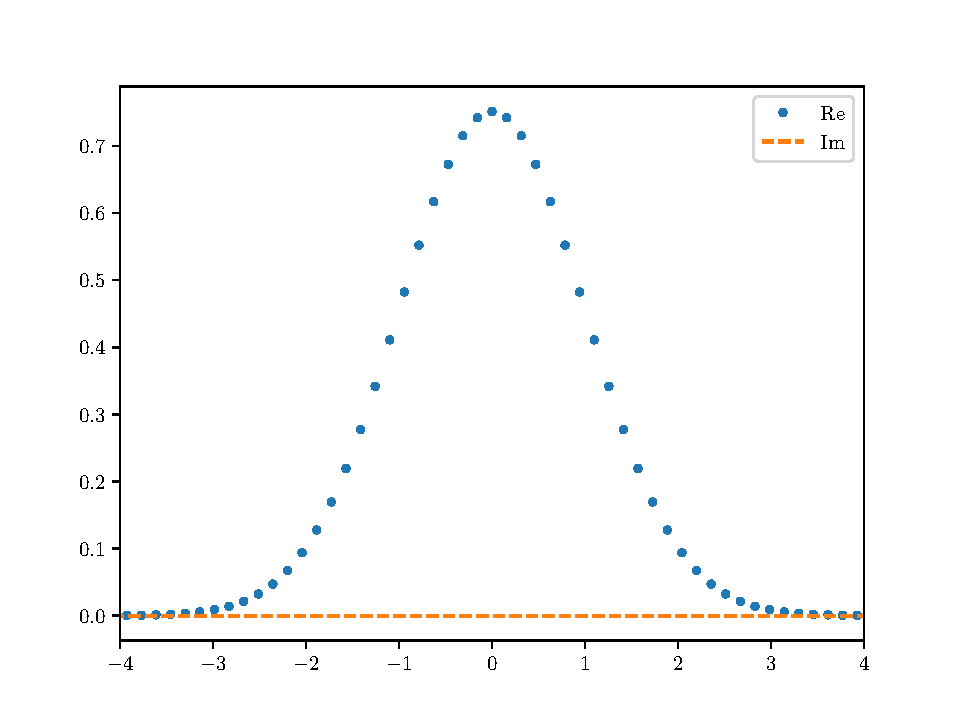
\includegraphics[width=\linewidth]{q1-2-0.pdf}
        \caption*{1023 grid points}
      \end{minipage}
      \begin{minipage}{0.32\linewidth}
        \centering
        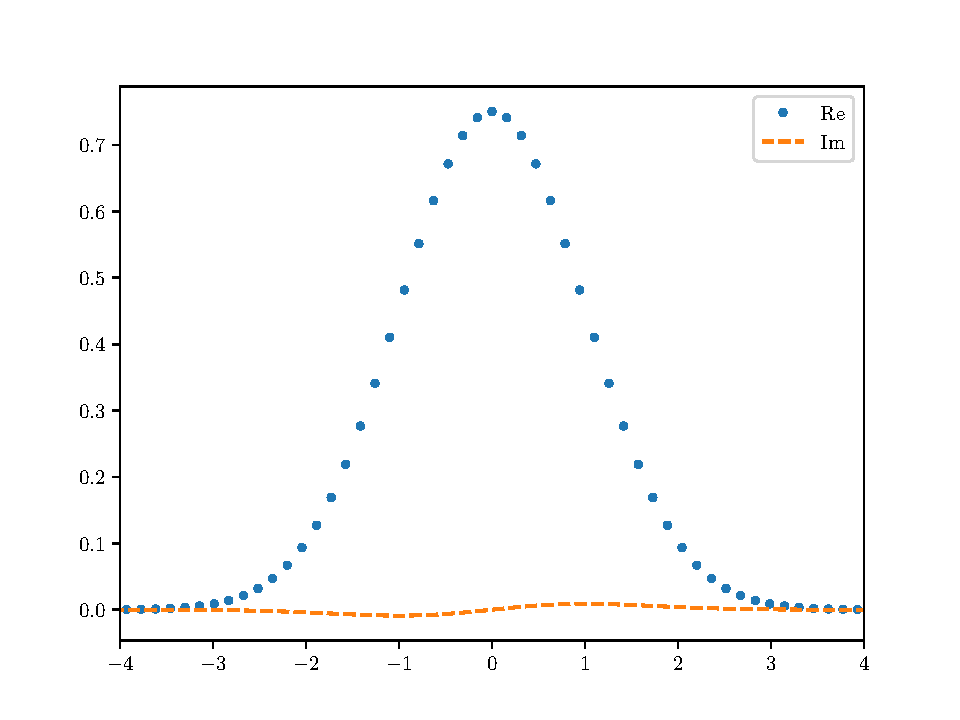
\includegraphics[width=\linewidth]{q1-2-1.pdf}
        \caption*{1024 grid points}
      \end{minipage}
      \begin{minipage}{0.32\linewidth}
        \centering
        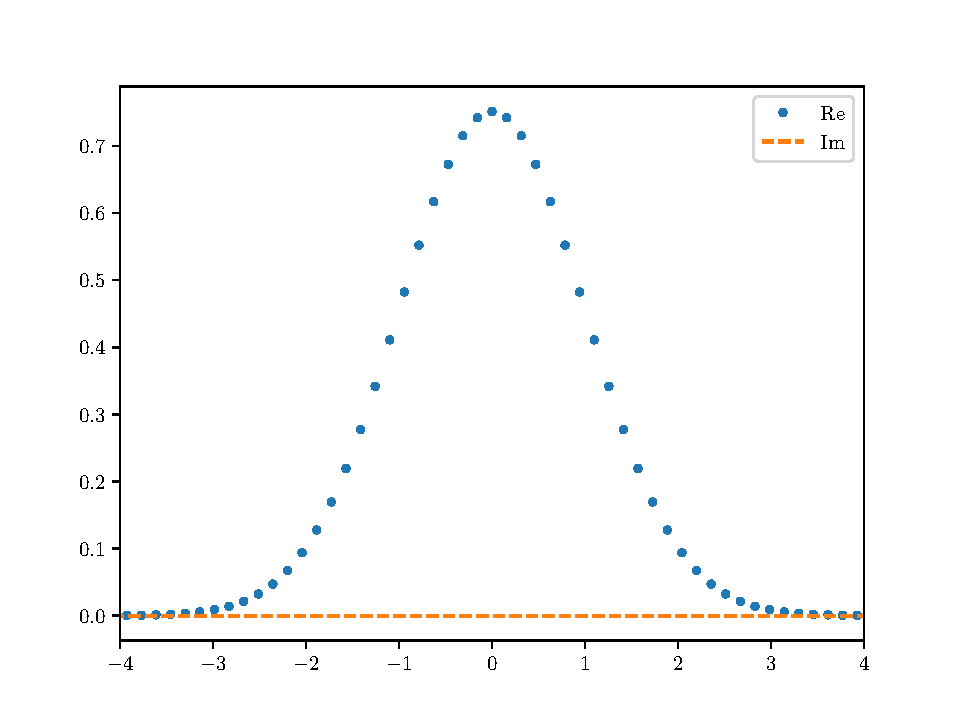
\includegraphics[width=\linewidth]{q1-2-2.pdf}
        \caption*{1025 grid points}
      \end{minipage}
      \caption{}
      \label{fig:1-2}
    \end{figure}

    Note that the relevant errors of $\Delta p$ are larger than the ones of $\Delta x$, and the when the number of grid points is odd the results are more accurate than the case that the number of grid points is similar but is even.
    This can be also justified the imaginary part of the wavefunction in momentum space.
        
    \item With 1024 gird points, the answer is 
    \begin{quotation}
      Potential: 0.25000000; Kinetic: 0.25097895; Total = 0.50097895.
    \end{quotation}
    With $2^{20} = 1048576$ gird points, the answer is
    \begin{quotation}
      Potential: 0.25000000; Kinetic: 0.25000095; Total: 0.50000095.
    \end{quotation}

    Note that the analytical expectation of the total energy is $0.5$.
  \end{enumerate}
  
  \item \begin{enumerate}[(i)]
    \item Use $2^{12} = 4096$ grid points uniformly spanned on $[-20,\ 20]$.  Results plotted in Figure~\ref{fig:2-1}.
    \begin{figure}[H]
      \centering
      \begin{minipage}{0.32\linewidth}
        \centering
        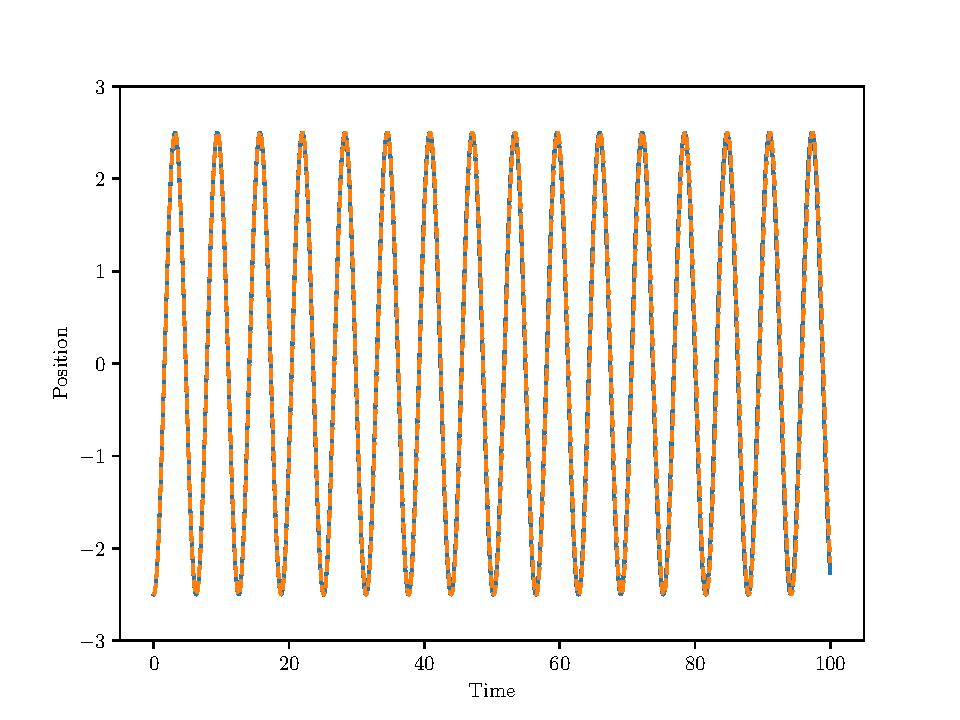
\includegraphics[width=\linewidth]{q2-1_time_position.pdf}
      \end{minipage}
      \begin{minipage}{0.32\linewidth}
        \centering
        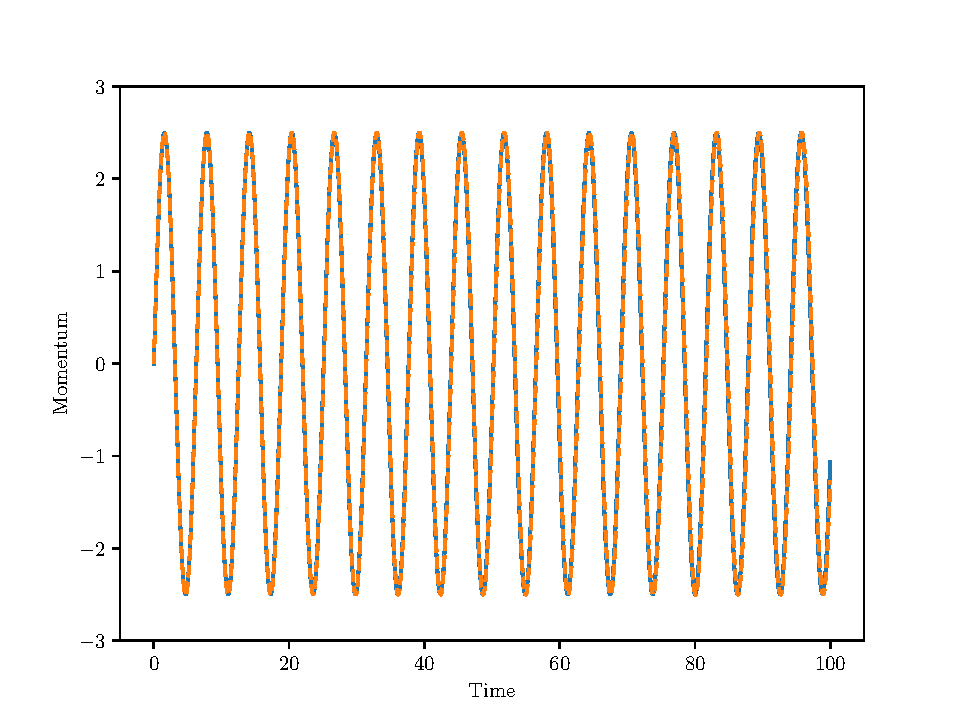
\includegraphics[width=\linewidth]{q2-1_time_momentum.pdf}
      \end{minipage}
      \begin{minipage}{0.32\linewidth}
        \centering
        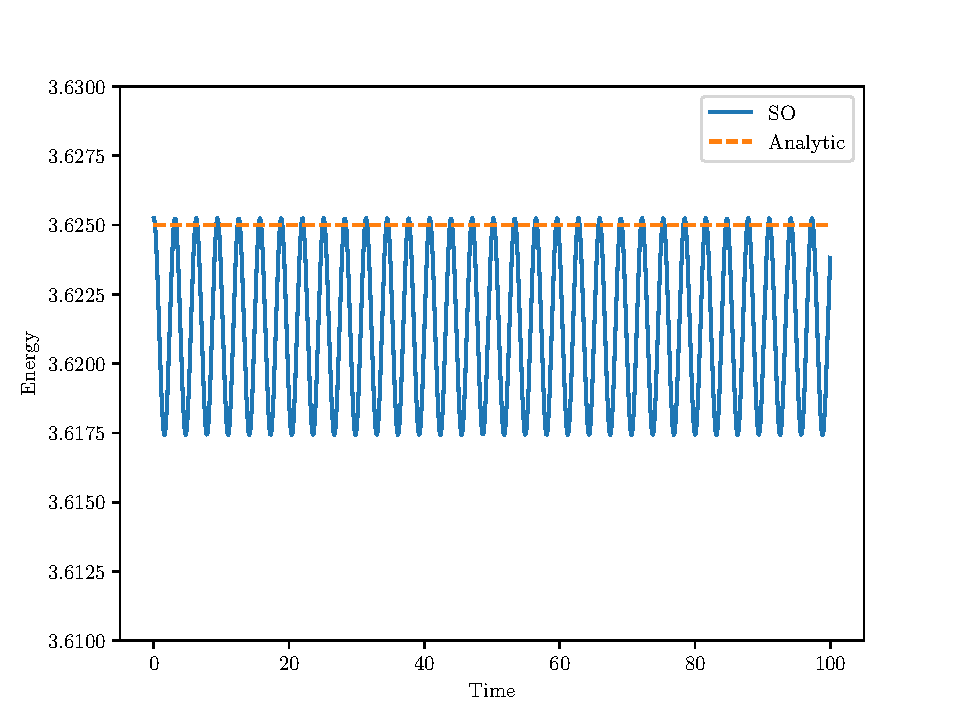
\includegraphics[width=\linewidth]{q2-1_time_energy.pdf}
      \end{minipage}
      \caption{}
      \label{fig:2-1}
    \end{figure}
    The movie is showed in \texttt{q2-1.mp4}.

    \item Still use $2^{12} = 4096$ grid points uniformly spanned on $[-20,\ 20]$.  Results plotted in Figure~\ref{fig:2-2}.
    \begin{figure}[H]
      \centering
      \begin{minipage}{0.32\linewidth}
        \centering
        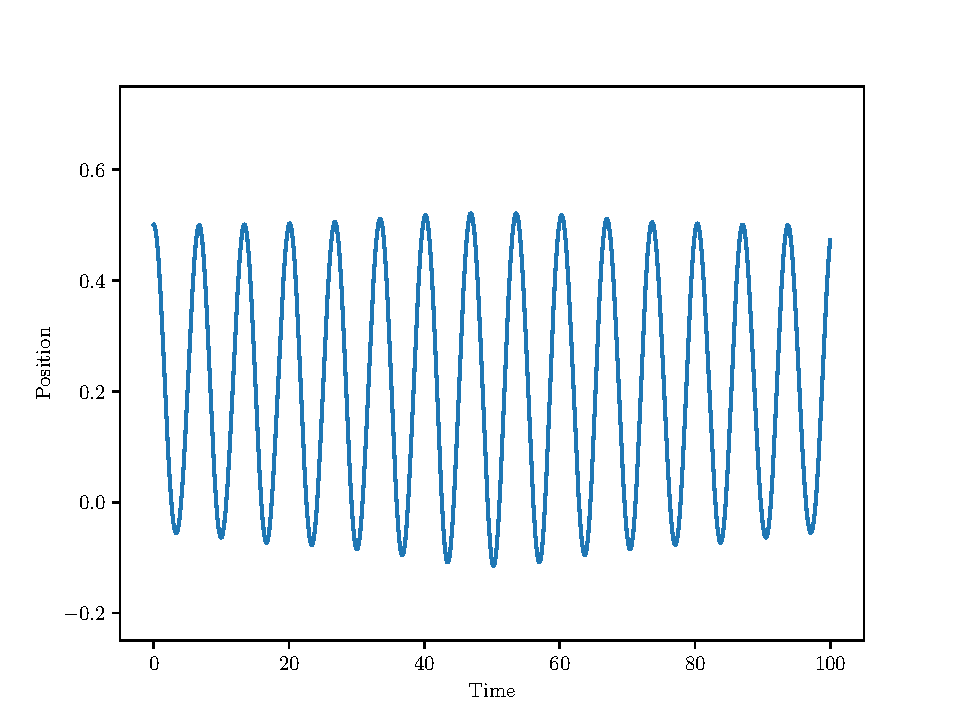
\includegraphics[width=\linewidth]{q2-2_time_position.pdf}
      \end{minipage}
      \begin{minipage}{0.32\linewidth}
        \centering
        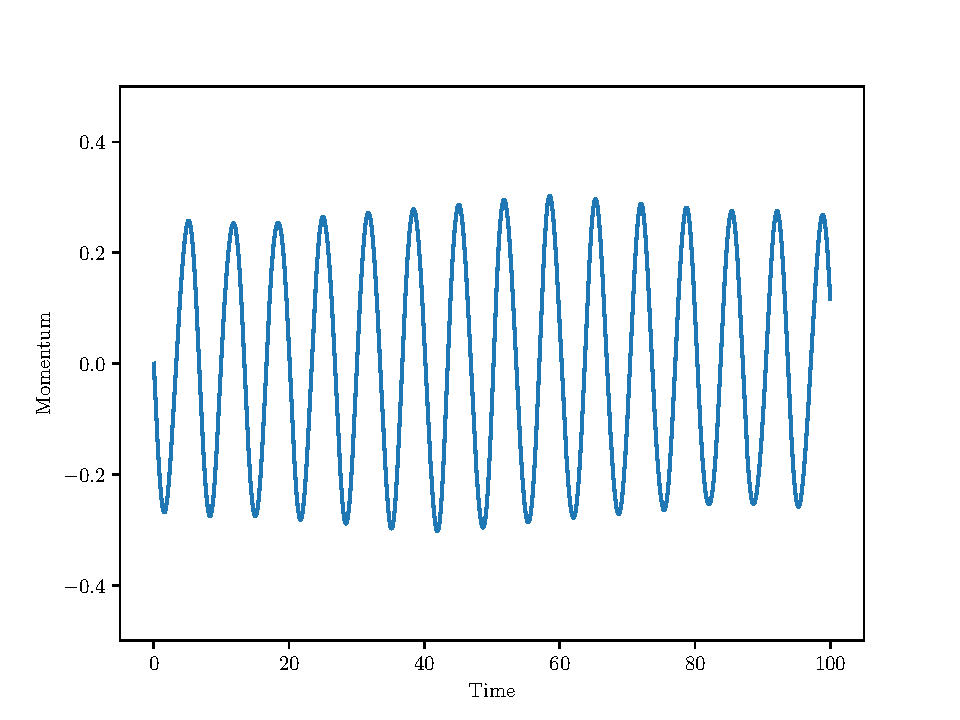
\includegraphics[width=\linewidth]{q2-2_time_momentum.pdf}
      \end{minipage}
      \begin{minipage}{0.32\linewidth}
        \centering
        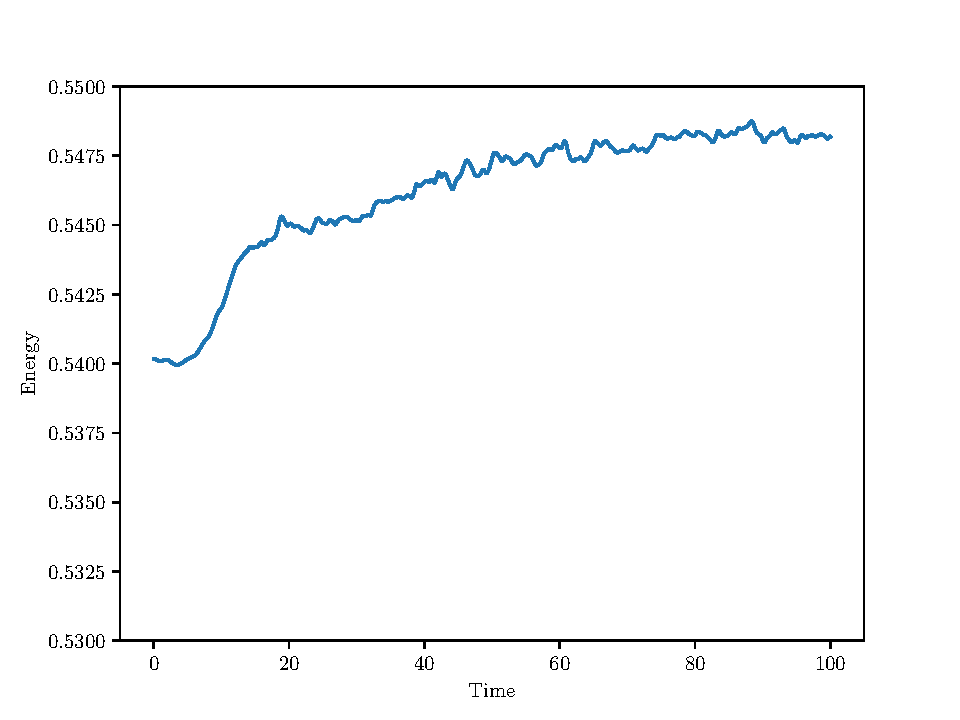
\includegraphics[width=\linewidth]{q2-2_time_energy.pdf}
      \end{minipage}
      \caption{}
      \label{fig:2-2}
    \end{figure}
    The movie is showed in \texttt{q2-2.mp4}.

    \item The energy of the ground state calculated by (Sine-)DVR (spanned on $[-20,\ 20]$ using 1024 basis) is 
    0.49218750 a.\,u., while imaginary time propagation SO (using grid basis spanned on $[-20,\ 20]$ with 4096 grid points) gives 0.49242469 a.\,u..
    The wavefunction of the ground state is plotted in Figure~\ref{fig:2-3}.
    \begin{figure}[H]
      \centering
      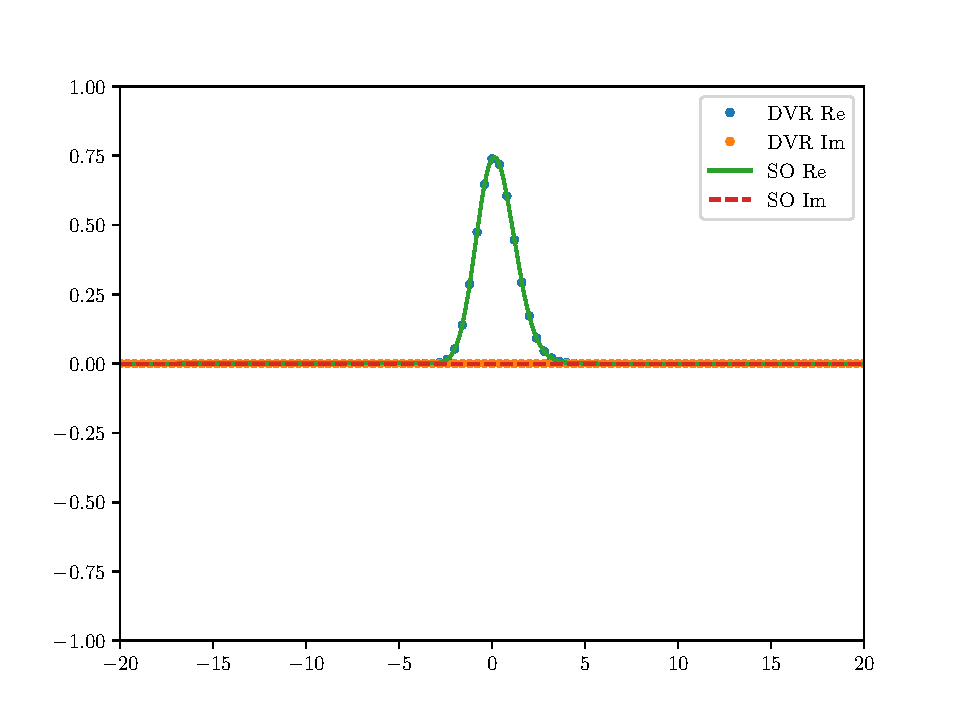
\includegraphics[width=0.6\linewidth]{q2-3.pdf}
      \caption{}
      \label{fig:2-3}
    \end{figure}
    
    \item Use $2^{12} = 4096$ grid points uniformly spanned on $[-20,\ 20]$. See \texttt{q2-4.mp4}. Note that the potential function used in the propagator $\tilde{V}(x) = V(x) - V_a(x)$ in order to absorb the wavefunction moved out from $[-10,\ 10]$.
  \end{enumerate}

  \item \begin{enumerate}[(i)]
    \item 1
    \item 2
    \item 3
  \end{enumerate}
\end{enumerate}

\end{document}


